\documentclass[12pt]{report}

\usepackage[utf8]{inputenc}
\usepackage{amsmath}
%\usepackage{ae}
\usepackage{graphicx}
\usepackage{color}
\usepackage{tikz}
\usepackage[tc]{titlepic}
\usepackage[toc,page]{appendix}

%\usepackage{bbm}
%\usepackage[swedish]{babel}
\newcommand{\N}{\ensuremath{\mathbbm{N}}}
\newcommand{\Z}{\ensuremath{\mathbbm{Z}}}
\newcommand{\Q}{\ensuremath{\mathbbm{Q}}}
\newcommand{\R}{\ensuremath{\mathbbm{R}}}
\newcommand{\C}{\ensuremath{\mathbbm{C}}}
\renewcommand{\d}{\ensuremath{\mathrm{d}}}
\newcommand{\e}{\ensuremath{\mathrm{e}}}
\renewcommand{\L}{\ensuremath{\mathcal{L}}}
\renewcommand{\i}{\ensuremath{i}}
\newcommand{\re}{\ensuremath{\mathrm{Re}}}
\newcommand{\im}{\ensuremath{\mathrm{Im}}}
\newcommand{\At}{\ensuremath{{A_x}}}
%\renewcommand{\i}{\ensuremath{\mathrm{i}}}
\newcommand{\ket}[1]{|#1\rangle}
\newcommand{\bra}[1]{\langle#1|}
\newcommand{\braket}[2]{\bra{#1}#2\rangle}
\newcommand{\bracket}[3]{\bra{#1}#2\ket{#3}}
\newcommand{\fig}[3]{
\begin{figure}
\centering
\includegraphics{figs/#1}
\caption{#2}
\end{figure}
}


\title{Holographic Methods for Condensed Matter Physics}
\author{Petter Säterskog}
\begin{document}

\titlepic{
\centering
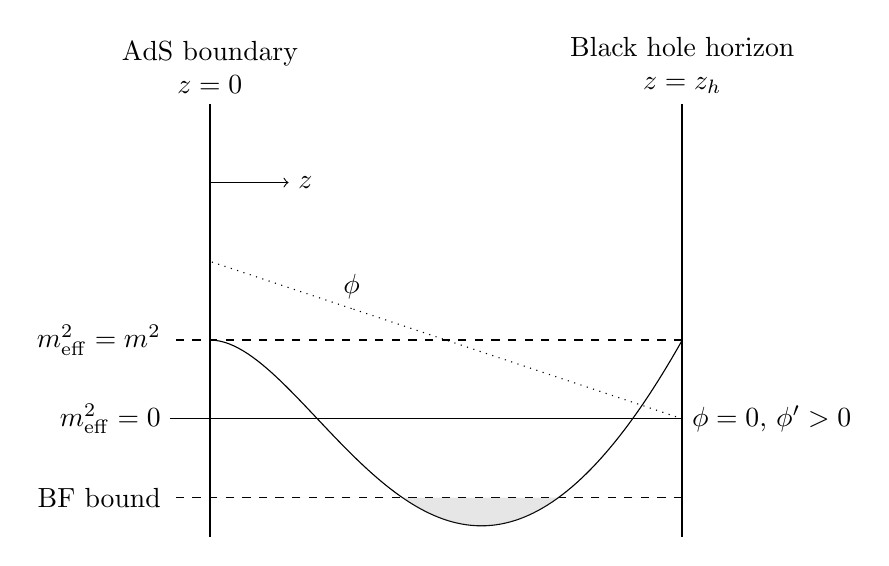
\begin{tikzpicture}
    \draw[->] (0,3) -- (1,3) node[right] {$z$};
    \draw[-,thick] (0,-1.5) -- (0,4) node[above,align=center] {AdS boundary\\$z=0$};
    \draw[-,thick] (6,-1.5) -- (6,4) node[above,align=center] {Black hole horizon\\$z=z_h$};
    \draw[-] (6,0) -- (-0.5,0) node[left] {$m_{\mathrm{eff}}^2=0$};
    \draw[-] (6,1) -- (-0.5,1)[dashed] node[left] {$m_{\mathrm{eff}}^2=m^2$};
    \draw[-] (6,-1) -- (-0.5,-1)[dashed] node[left] {BF bound};
    \draw[dotted] plot[domain=1:0.3,samples=50] (\x*6,{2*(1-\x)})node[above] {$\phi$};
    \draw[dotted] plot[domain=0.3:0,samples=50] (\x*6,{2*(1-\x)});
    \draw[-] (6,0) node[right] {$\phi=0$, $\phi^\prime>0$};
    \draw[solid] plot[domain=0:1,samples=100] (\x*6,{1-2*\x*\x/(1-\x*\x*\x)*4*(1-\x)*4*(1-\x)});
    \draw [fill=gray,fill opacity=0.2,draw=none] plot[domain=0:1,samples=100] (\x*6,{-1}) -- plot[domain=0:1,samples=100] (\x*6,{min(1-2*\x*\x/(1-\x*\x*\x)*4*(1-\x)*4*(1-\x),-1)});
\end{tikzpicture}
}
\maketitle
\section*{Acknowledgements}
Thanks Mum.
\tableofcontents
\chapter{Introduction}
The AdS-CFT correspondence was conjectured in 1997 \cite{Maldacena:1997re}. It relates the physics of a string theory in Anti de Sitter space (AdS) to a conformal field theory (CFT) on the boundary of the AdS space.

\section{The Correspondence\label{correspondence}}
The correspondence can be formulated by the GKPW equation \cite{Witten:1998qj}
\begin{equation}
 Z_{\text{CFT}}=Z_{\text{strings}}
\label{GKPW}
\end{equation}
where $Z_{\text{CFT}}$ is the partition function of the boundary theory and $Z_{\text{strings}}$ is the partition function of the bulk theory. The relation between the Lagrangians of the theories is unknown but the boundary values of fields in the bulk theory correspond to fields in the CFT.
TODO
Lorentz invariance, relativity, causality, locality?
\section{Applications}
Strong coupling
Quark-Gluon plasma
High TC Superconductors, Graphene.
Inverse, Cosmology?

\chapter{Application to Two-Dimensional Condensed Matter Systems}
We wish to model a high temperature superconductor. Conventional superconductors are well described by the BCS theory where the electrons, photons and phonons are the degrees of freedom of interest. The importance of the phonon interactions was understood from the isotope effect, the mass of the atoms in the lattice changed the superconductivity behavior. The isotope effect is though much weaker, TODO cite, in high temperature superconductors and the phonons are thus not believed to be important for high temperature superconductivity. The important degrees of freedom are the electrons and the photons. The electrons are, just as in BCS theory, expected to form Cooper-pairs, TODO cite. These are pairs of electrons of opposite spin but otherwise in the same state effectively becoming spin 0 particles. Our high temperature superconductor model will thus contain two fields, a spin 1 field $A_a$ for the photons and a spin 0 field $\psi$ for the Cooper-pairs.
\section{Symmetry Assumptions}
Gauge symmetry, say that $\psi$ is complex
Translational invariance...
\section{A Lagrangian}
There are many different ways to construct a bulk Lagrangian for the fields $A_a$ and  $\psi$ and the metric $g_{ab}$. A Lagrangian previously used succesfully to model two-dimensional electron condensates\cite{hartnoll9},\cite{horowitz} will initially be used here.
\begin{eqnarray}
 \mathcal{L}=&\frac{1}{2\kappa}\left(R-2\Lambda\right)-\frac{1}{4}F_{ab}F^{ab}-m^2|\psi|^2-|D_a\psi|^2
\label{L}
\end{eqnarray}
This is obtained using Wilsonian naturalness meaning that the lowest order terms obeying all symmetries are used. A higher order term will be investigated in \ref{higherOrder}.\\

The action $S$ is calculated from this Lagrangian from
\begin{equation}
 S=\int\d^{d+1} x\sqrt{g}\L+S_\mathrm{boundary}.
\end{equation}
where $g$ is the absolute value of the determinant of the metric tensor, $g=|\det g_{ab}|$. $S_\mathrm{boundary}$ is a boundary term that later will be determined. It doesn't affect the equations of motion but is needed for getting normalizeable modes.\\

The first term of the Lagrangian is an Einstein-Hilbert term with a cosmological constant $\Lambda$. A negative cosmological constant gives a asymptotically anti-de-Sitter space as required. $R$ is the Ricci scalar curvature obtained from the nmetric $g_{ab}$. The constant $\kappa$ determines the coupling between the metric and the other fields.\\

The second term is an ordinary Maxwell term where $F_{ab}=\nabla_aA_b-\nabla_bA_a$. The spacetime will not be flat so covariant derivatives have to be used. See Appendix \ref{conventions}.\\

The third and fourth terms are the kinetic and mass terms for the scalar field respectively. $D_a$ is the gauge covariant derivative $D_a=\nabla_a-iqA_a$. This makes the Lagrangian invariant under a U(1) gauge transformation
\begin{eqnarray}
 \psi&\rightarrow&\mathrm{e}^{i\theta(x)}\psi\\
 A_a&\rightarrow& A_a+\frac{1}{q}\nabla_a\theta(x)\label{Agauge}.
\end{eqnarray}
This Lagrangian also possess conformal invariance. This means that the Lagrangian is unchanged by the transformation $g_{ab}\rightarrow f(x)g_{ab}$. TODO check.
The Lagrangian is also manifestly Lorentz invariant imposing Lorentz invariance of the boundary theory. 
\section{Equations of Motion}
Varying the fields gives the equations of motion. First vary $\psi$. This gives
\begin{equation}
\begin{split}
\left(m^2-\nabla^2-q^2A^2+\i q(\nabla_aA^a)\right)\psi&=0.
\end{split}
\end{equation}
Varying $A_a$ gives these equations of motion
\begin{equation}
 -\nabla_aF^{ab}+2q^2|\psi|^2A^b+iq\left(\overline{\psi}\nabla^b\psi-\psi\nabla^b\overline{\psi}\right)=0
\end{equation}
A real $\psi$ simplifies calculations and that can be obtained since the gauge invariance lets us relate any configuration with a real one through a gauge transformation. The Lorentz gauge,
\begin{equation}
 \nabla_aA^a=0\label{lorentz},
\end{equation}
removes the last term in the parenthesis of the equation of motion for $\psi$. The equation of motion for $\psi$ does not mix the real and imaginary parts after this choice and $\psi$ can be taken to be real since a global shift of phase does not affect $A_a$, see \eqref{Agauge}. The gauge is still not completely fixed, a gauge transformation $\theta(x)$ such that $\nabla_a\nabla^a\theta(x)=0$ can still be done without violating the gauge condition, \eqref{lorentz}. The equations of motion are
\begin{equation}
\begin{split}
\left(m^2-\nabla^2-q^2A^2\right)\psi&=0\\
-\nabla_aF^{ab}+2q^2|\psi|^2A^b&=0.
\end{split}
\end{equation}
after choosing the Lorentz gauge and a real $\psi$.
\section{Parameters}
There are multiple unknown parameters. These must be investigated to find values that give us the boundary theory we are interested in. The Lagrangian contains the parameters $\kappa$, $\Lambda$, $m^2$, $q$. Some of these parameters might be redundant since we can make different symmetry transformations of fields and coordinates. The physics of the bulk are treated in the classical limit and the Lagrangian can thus be changed as long as the equations of motion for $\psi$ and $A_a$ are left unchanged.
\subsection{$\kappa$}
The Einstein-Hilbert term of the Lagrangian makes the theory gravitational. $\kappa$ is proportional to Newton's gravitational constant. A small $\kappa$ gives the probe limit where the metric equations of motion can be solved independently of the other fields. This can be understood by varying the Lagrangian with respect to the metric, the Einstein-Hilbert part gives a term inversely proportional to $\kappa$ and the rest of the Lagrangian gives the stress-energy tensor

This greatly simplifies calculations and will therefore be used throughout this work. It is though not guaranteed that interesting boundary theories are dual to bulk theories in the probe limit. Earlier studies have though found that interesting boundary systems can be obtained by treating a bulk in the probe limit. A superconducting condensate developes for low temperatures in the work by S. Hartnoll, C. Herzog and G. Horowitz \cite{hartnoll9} where the bulk is treated in the probe limit. $\kappa\rightarrow0$ is a fixed-point of the theory so the physics is independent of the exact value of $\kappa$ as long as we are in the probe limit.
\subsection{$\lambda$}
Scale-invariance of the system lets us choose an arbitrary $\lambda$. Two systems with different $\lambda$ can be shown to be equal by a rescaling. $\lambda$ sets a scale to which other parameters, e.g $m^2$, can be related. Scale-invariance can thus not be used to choose those parameters freely.\\
$\lambda$ will be set to a convenient number in numerical calculations but kept in calculations for clarity.



\subsection{$q$}
Considering $\tilde{\psi}=q\psi$ and $\tilde{A}_a=qA_a$ as the fields gives a Lagrangian of the same form but with different constants $\alpha_1$ and the whole Lagrangian is divided by $q^2$ except for the term originally containing $q^2$ which is divided by $q^4$. Multiplying the Lagrangian by a constant doesn't affect the equations of motion so $q=1$ can be assumed without getting a less general Lagrangian. It should be noted that a different value of $q$ would give $q\psi$ as solution instead where $\psi$ is the solution of the equations of motion when $q=1$. The same is true for $A_a$.\\
\subsection{$m^2$}
$m$ is the mass of the scalar field in the bulk. What values of $m$ that are suitable will be investigated later when solving the equations of motion in the bulk.

The bulk field equations are obtained by varying the bulk Lagrangian with respect to all the fields. This can be done with the Euler-Lagrange equation since the action does not contain any higher derivatives. The Euler-Lagrange equation for a scalar field $\At$ states
\begin{equation}
 \partial_a\left(\frac{\partial\mathcal{L}}{\partial(\partial_a\At)}\right)-\frac{\partial\mathcal{L}}{\partial\At}=0.
\end{equation}
$\At$ is 0 at the horizon but increases as $\psi$ is non-zero. This effective mass breaks the BF bound since $g^{tt}$ diverges at the horizon. TODO, talk to Ulf and do calculations.

\section{Partition Function}
The partition function is a concept from statistical physics. It is for a quantum-mechanical system defined as
\begin{equation}
 Z(\beta)=\mathrm{tr}(\e^{-\beta\hat{H}})
\end{equation}
where $\hat{H}$ is the time-independent Hamiltonian and $\beta=(k_BT)^{-1}$ where $k_B$ is Boltzmann's constant and $T$ is the temperature. Hereafter we let $k_B=1$ meaning that we measure temperature in units of what energy it corresponds to. The partition funciton is similar to the trace of the time-evolution operator $\hat{U}(t_2,t_1)$ evolving a state from time $t_1$ to $t_2$
\begin{equation}
 \mathrm{tr}(\hat{U}(t_2,t_1))=\mathrm{tr}(\e^{-\i\frac{(t_2-t_1)\hat{H}}{\hbar}})=f(t_2-t_1).
\end{equation}
We will hereafter let $\hbar=1$ by measuring energy in units of inverse time. The partition function can then be obtained as the analytical extension of $f$,
\begin{equation}
 Z(\beta)=f(-\i\beta).
\end{equation}
The trace of the time evolution operator can be calculated as an integral over configuration space which in our case will be fields configurations $\Psi$,
\begin{equation}
 f(t)=\int \mathcal{D}[\Psi] \bracket{\Psi}{\hat{U}(t,0)}{\Psi}.
\end{equation}
The time-evolution operator matrix elements can be calculated using Feynman's path integrals \cite{feynman1965quantum},
\begin{equation}
 \bracket{\Psi_2}{\hat{U}(t,0)}{\Psi_1}=\int_{\Psi_1}^{\Psi_2} \mathcal{D}[\Psi(t)]\e^{\i S[\Psi(t)]}
\end{equation}
where $S[\Psi(t)]$ is the action of the path $\Psi(t)$ through field configurations. Combining these results tells us that the trace $f(t)$ can be calculated as a periodic time path integral with period $t$
\begin{equation}
 f(t)=\int_0^t \mathcal{D}[\Psi(t)]\e^{\i S[\Psi(t)]}.
\end{equation}
This means that $Z(\beta)$ can be obtained by calculating a path integral where the time is imaginary and periodic. The action must be analytically extended to imaginary time $\tau=\i t$.
\begin{equation}
 S[\Psi(\tau)]=\int_0^\beta\d \tau\int\d x\sqrt{g} \L(\Psi(\tau),\Psi^\prime(\tau),...)
\end{equation}
The CFT we are interested in lives on the boundary of an AdS theory. The metric of the CFT is the metric induced from the bulk theory. The boundary is time-like and the time periodicity of the two theories are thus the same. This means that they are at the same temperatures.\\

The functional derivative of the action is just the ordinary derivative of the Lagrangian function. TODO
The partition function is in the classical limit
\begin{equation}
 Z(\beta)=f(-\i\beta)\stackrel{\mathrm{classical}}{=} \e^{i S_c}\label{classical}
\end{equation}
where $S_c$ is the action of classical periodic path with period $-\i\beta$.
\section{Field Theory Expectation Values}
The boundary values of the bulk fields correspond to fields in the CFT. Expectation values of observables in the CFT can be calculated using a generating functional $Z[J]$. This is a partition function for a system with a perturbed Lagrangian $\L_J(x)=\L(x)+J(x)O(x)$. Here $O(x)$ is a local operator on the fields. The generating functional can be regarded an expectation value of a system with the original Lagrangian $\L$.
\begin{equation}
\begin{split}
 Z[J]&=\int_0^{-\i\beta} \mathcal{D}[\psi(t)]\e^{\i \int \L(\psi(x))+J(x)O(\psi(x))}\\
&=Z[0]\int_0^{-\i\beta} \mathcal{D}[\psi(t)]\frac{\e^{\i\int \L(\psi(x))}}{Z[0]}\e^{\i\int J(x)O(\psi(x))}\\
&=Z[0]\langle\e^{\i\int J(x)O(\psi(x))}\rangle
\end{split}
\end{equation}
Taking a functional derivative of this gives:
\begin{equation}
\begin{split}
 \frac{\delta}{\delta J}\log(Z[J])|_{J=0}&=\frac{Z[0]\langle\i O(\psi(x))\e^{\i\int J(x)O(\psi(x))}\rangle}{  Z[0]\langle\e^{\i \int J(x)O(\psi(x))}\rangle }\big |_{J=0}\\
&=\i \langle O(\psi(x))\rangle\label{expectation}
\end{split}
\end{equation}
The partition functions of the bulk and boundary theories are the same even for a perturbed Lagrangian. Both Lagrangians are then perturbed. Expectation values of operators of the boundary theory can thus be calculated using the partition function for the bulk theory. It is though not trivial to figure out what fields in the bulk theory corresponds to what operators in the boundary theory. The next chapter will show how to solve the bulk theory and obtain CFT observables.
\chapter{Solution of the Classical Bulk Theory}
We wish to compute expectation values of the CFT. This will be done through the correspondence \eqref{GKPW}. Then bulk theory must then be solved. The bulk theory was assumed to be classical in Section \ref{correspondence} so the system is solved by finding the equations of motion for the fields and solving them. This lets ut calculate the partition function and using it to find CFT expectation values through \ref{expectation}.
\section{Limitations}
The Lagrangian describes a general system so there are many solutions to the equations of motion. We wish to investigate two properties of a superconductor, the development of a condensate at low temperatures and the conductivity at different frequencies. We are interested in a superconductor subject to spatially uniform conditions, the applied electric field is uniform and the chemical potential is uniform. The atomic lattice and its imperfections are thus not accounted for but interesting superconductivity behaviour has been obtained anyways \cite{hartnoll9}.\\

It is thus enough to look at a system with translational symmetry in the $x$ and $y$ directions.\\

The conductivity is the electrical current response to an applied electrical field. The applied electric field is infinitesimal so we will solve the non-linear field equations without it and then add it as a perturbation. The non-linear system is thus also rotationally symmetric. The superconductor is subject to conditions constant in time except for the applied electrical field, e.g. no time-dependent chemical potential. This lets us assume time-independence while solving the non-linear field equations. 
\section{Metric}
The Lagrangian, \eqref{L}, contains an Einstein-Hilbert term with a cosmological constant.
\begin{equation}
\Lambda=-\frac{3}{L^2}
\end{equation}
where $L$ is a length.
A Gibbons-Hawking-York boundary term is also needed \cite{PhysRevD.15.2752}, \cite{PhysRevLett.28.1082} TODO, read, comment.
\begin{equation}
 S_{\mathrm{grav}}=\frac{1}{2\kappa}\int \d^{d+1}x\sqrt{-g}\left(R-2\Lambda\right)-\frac{1}{\kappa}\int \d^dx\sqrt{\gamma}\left(-\gamma^{ab}\nabla_an_b+\frac{d-1}{L}\right)
\end{equation}
%Here $R$ is the Ricci scalar. The gravitational constant $\kappa$ (related to Newton's constant by $\kappa=8\pi G$) is assumed to be small so that we are in a so called ``probe limit''. We will later see when this assumption can't be trusted.
$n_a$ is a normal vector at the boundary. The bulk equation of motion for the metric $g_{ab}$ is Einstein equation with a cosmological constant
\begin{equation}
R_{ab}-\frac{1}{2}g_{ab}R+g_{ab}\lambda=\kappa T_{ab}
\end{equation}
where $R_{ab}$ is the Ricci curvature tensor and $T_{ab}$ is the energy-momentum tensor. We assumed the probe limit in Section \ref{kappa} and therefore neglect the right hand side of this equation. We thus seek a vacuum solution to Einsteins equation with a negative cosmological constant. We want a translationally invariant solution in the $t$, $x$, and $y$ directions.
The probe limit lets us solve the equations of motion for the metric independently of the other fields. We are looking for an equilibrium solution at a finite temperature $T$ and the solution is then known to be a black hole(TODO ref), the Schwarzschild metric in AdS space. The metric has the following form in a particular choice of coordinates where the radial coordinate $z$ is 0 at the boundary and $z_h$ at the horizon
\begin{equation}
 g_{ab}\d x^a\d x^b=\frac{L^2}{z^2}\left(\frac{\d z^2}{f(z)}-f(z)\d t^2+\d \mathbf{x}^2\right).\label{metric}
\end{equation}
Here $f(z)=1-z^dz_h^{-d}$. The vector $\mathbf{x}$ thus has $d-1$ components. $f(z)$ approaches 1 at the boundary and the space is asymptotically AdS.\\
All coordinates are evidently of the same unit. The gravitational part of the Lagrangian can now be removed and this background metric can be used instead of solving the equations of motion for the metric together with the fields. This gravitational part of the Lagrangian must though be kept when calculating the value of the total action. The Ricci scalar of this metric is
\begin{equation}
 R=-\frac{d(d+1)}{L^2}=2\Lambda\frac{d+1}{d-1}
\end{equation}
TODO: does the region behind the horizon contribute?
The action can be calculated using this. Consider the space $(z,t,\mathbf{x})\in[\epsilon,z_h]\times V$ corresponding to a $d$-volume of the boundary theory $V$. The action boundary density is then
\begin{equation}
\begin{split}
 \frac{S_{\mathrm{grav}}}{V}&=\frac{\Lambda}{\kappa}\left(\frac{d+1}{d-1}-1\right)\int_\epsilon^{z_h}\d z\sqrt{-g}+
\frac{1}{\kappa}\sqrt{\gamma}\left(-\gamma^{ab}\partial_a\d z_b+\frac{d-1}{L}\right)\\
&=\frac{\Lambda}{\kappa}\frac{2}{d-1}\int_\epsilon^{z_h}\d z\left(\frac{L}{z}\right)^{d+1}+
\frac{1}{\kappa}\left(\frac{\epsilon}{L}\right)^{-d}\frac{d-1}{L}\\
&=\frac{L\Lambda}{\kappa}\frac{2}{d(d-1)}\left(\left(\frac{\epsilon}{L}\right)^{-d}-\left(\frac{z}{L}\right)^{-d}\right)\\
&=-\frac{1}{L\kappa}\left(\left(\frac{\epsilon}{L}\right)^{-d}-\left(\frac{z_h}{L}\right)^{-d}\right)
\end{split}
\end{equation}

The total action density is obtained as $\epsilon\rightarrow0$.
.  TODO, imaginary time, deficit angle gives $T$.

The horizon $z_h$ and the curvature length $L$ set length scales in the metric. Length units in the numerical solution can be chosen such that $z_h=1$. This means that we for different temperatures have different units since $z_h$ is related to the temperature. We will have to convert between these units when comparing results from different temperatures.\\

\begin{equation}
 T=\frac{d}{4\pi  z_h}\label{T}
\end{equation}
%This $T$ in units of energy is also in units of inverse length since we chose the energy unit to the inverse time it 
\section{Equations of Motion}
First consider a system with $A_x=A_y=0$. The field equations obtained by varying the fields $\psi$, $\At$ are respectively
\begin{eqnarray}
0=&\psi \left(- \frac{m^{2}}{\operatorname{f}\left(r\right)} + \frac{\phi^{2}}{\operatorname{f}^{2}\left(r\right)}\right) + \frac{\partial^{2}}{\partial^{2} r}  \psi\nonumber\\&+\left(\frac{\frac{\partial}{\partial r} \operatorname{f}\left(r\right)}{\operatorname{f}\left(r\right)} + \frac{2}{r}\right) \frac{\partial}{\partial r} \psi
\end{eqnarray}
\begin{eqnarray}
0=&- 2 \frac{\phi \psi^{2} r^{2}}{\operatorname{f}\left(r\right)} + r^{2} \frac{\partial^{2}}{\partial^{2} r}  \phi + 2 r \frac{\partial}{\partial r} \phi.
\end{eqnarray}
TODO, boundary conditions.\\
These equations have the trivial solution
\begin{equation}
 \begin{split}
  \psi=&0\\
  \At=\mu-\mu\frac{z}{z_h}\label{trivial}
 \end{split}
\end{equation}
\subsection{Choice of scalar mass $m$}
The mass squared of a scalar field in flat space must be non-negative for stability. This is though not the case in a space with negative curvature. The Breitenlohner-Freedman bound (BF) is a lower bound on $m^2$ of a massive scalar field in AdS space. It requires
\begin{equation}
 L^2m^2\geq-\frac{d^2}{4}\label{BF}
\end{equation}
for stability\cite{Kleban:2004bv}. The scalar field $\psi$ should obey this bound far away from the black-hole for normalizeable modes, TODO explain. We would though like a spontanous symmetry breaking of $\psi$ near the black hole (low energies) corresponding to the electron condensate \cite{Gubser:2008px}. This can happen because the coupling of $\psi$ to $A_a$ gives $\psi$ an effective mass that might break the BF bound near the black hole. \\The effective mass is given by:
\begin{equation}
 m_{\mathrm{eff}}^2=m^2+A_aA^a
%=m^2+g^{tt}\At^2
=m^2-\frac{z^2}{L^2(1-z^dz_h^{-d})}\At^2
\label{meff}
\end{equation}
This can for large enough values of $\At$ break the BF-bound, see Fig. \ref{BF}.
\begin{figure}
\centering
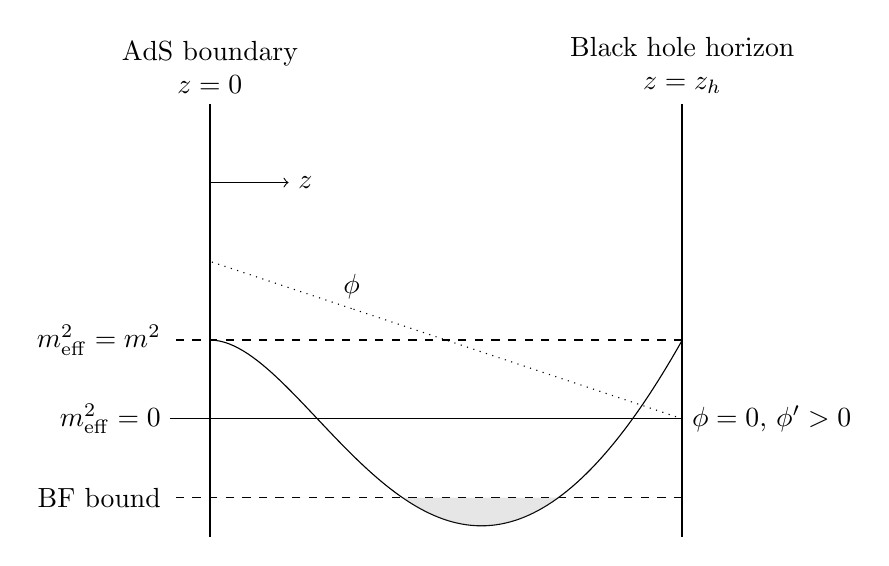
\begin{tikzpicture}
    \draw[->] (0,3) -- (1,3) node[right] {$z$};
    \draw[-,thick] (0,-1.5) -- (0,4) node[above,align=center] {AdS boundary\\$z=0$};
    \draw[-,thick] (6,-1.5) -- (6,4) node[above,align=center] {Black hole horizon\\$z=z_h$};
    \draw[-] (6,0) -- (-0.5,0) node[left] {$m_{\mathrm{eff}}^2=0$};
    \draw[-] (6,1) -- (-0.5,1)[dashed] node[left] {$m_{\mathrm{eff}}^2=m^2$};
    \draw[-] (6,-1) -- (-0.5,-1)[dashed] node[left] {BF bound};
    \draw[dotted] plot[domain=1:0.3,samples=50] (\x*6,{2*(1-\x)})node[above] {$\phi$};
    \draw[dotted] plot[domain=0.3:0,samples=50] (\x*6,{2*(1-\x)});
    \draw[-] (6,0) node[right] {$\phi=0$, $\phi^\prime>0$};
    \draw[solid] plot[domain=0:1,samples=100] (\x*6,{1-2*\x*\x/(1-\x*\x*\x)*4*(1-\x)*4*(1-\x)});
    \draw [fill=gray,fill opacity=0.2,draw=none] plot[domain=0:1,samples=100] (\x*6,{-1}) -- plot[domain=0:1,samples=100] (\x*6,{min(1-2*\x*\x/(1-\x*\x*\x)*4*(1-\x)*4*(1-\x),-1)});
\end{tikzpicture}
\caption{Schematic plot of how the the effective mass breaks the BF bound outside the horizon. A value of $\At$ has been assumed.\label{BF}}
\end{figure}
Consider the trivial, uncondensed, solution \eqref{trivial}. When does this give an effective mass breaking the BF-bound and possibly enabling an additional condensed solution? The location of the effective mass minimum, $z_0$, can be found by differentiating \eqref{meff} by $z$ and using \eqref{trivial},
\begin{equation}
\frac{z_0}{z_h}=\frac{1}{3} \left(\sqrt[3]{37+9 \sqrt{17}}-\frac{2}{\sqrt[3]{37+9 \sqrt{17}}}-2\right).
\end{equation}
The effective mass breaks the BF-bound at $z_0$ when
\begin{equation}
 \frac{\mu}{T}>
\frac{2\pi }{\sqrt{3}} \sqrt{\frac{4 L^2 m^2+9}{8-\sqrt[3]{142-34
   \sqrt{17}}-\sqrt[3]{142+34 \sqrt{17}}}}
\end{equation}
where \eqref{T} has been used.

\section{Boundary Behavior of Bulk Fields}
The bulk Lagrangian considered will contain different fields and depends both on the fields and their first derivatives. Consider a field $\psi$ with a kinetic term $-(\partial_a\psi)^2$ and a potential term $V(\psi)$. The classical solution is the one that extremizes the action. The action integral contains the metric as an integration measure
\begin{equation}
 S=\int\d^{d+1} x\sqrt{|\det g_{ab}|}\L\equiv\int\d^{d+1} x\sqrt{g}\L.
\end{equation}
The Euler-Lagrange equation is obtained by varying the action. The integration measure can then be regarded as part of the Lagrangian or covariant derivatives can be used in the derivation of the Euler-Lagrange equation. The measure becomes when using the metric \eqref{metric} $L^{d+1}z^{-d-1}$. The Euler-Lagrange equation gives
\begin{equation}
\begin{split}
 0=\partial_a\left(\frac{\partial (z^{-d-1}(V(\psi)-(\partial_b\psi)^2)) }{\partial(\partial_a\At)}\right)-\frac{\partial  (z^{-d-1}(V(\psi)-(\partial_b\psi)^2) )}{\partial\At}=\\
 =-\partial_a\left(z^{-d-1}2\partial^a\psi\right)-z^{-d-1}V'(\psi)\\
\end{split}
\end{equation}
We will be interested in boundary systems with translational symmetry so $\psi$ is assumed to be a function of $z$, TODO motivate more. The equation of motion then becomes
\begin{equation}
\begin{split}
0=-\partial_z\left(z^{-d-1}2g^{zz}\partial_z\psi\right)  -\frac{V'(\psi)}{z^{d+1}}=\\
-\partial_z\left(z^{-d-1}2(z^2L^{-2}f(z))\partial_z\psi\right)  -\frac{V'(\psi)}{z^{d+1}}=\\
-z^{-d-1}2z^2L^{-2}f(z)\psi''-L^{-2}\left((-d+1)z^{-d}2f(z) + z^{-d+1}2f'(z)\right)\psi' -\frac{V'(\psi)}{z^{d+1}}
\end{split}
\end{equation}
This gives a second order differential equation for $\psi(z)$
\begin{equation}
\begin{split}
0=-z^22f(z)\psi''-\left((-d+1)z2f(z) + z^22f'(z)\right)\psi' -L^2V'(\psi)
\end{split}
\end{equation}
Now consider the boundary, $z=0$. Our metric is required to be asymptotically AdS so $f(0)\rightarrow1, zf'(0)\rightarrow0$. $\psi$ can be expanded at the boundary as a Laurent series. Call the lowest exponent in this series $\Delta$. $\psi$ will then behave as $z^\Delta$ near the boundary. This should solve the differential equation in the near boundary limit. Insertion of $z^\Delta$ into the differential equation and taking the limit of small $z$ gives
\begin{equation}
\begin{split}
0&=-z^22\Delta(\Delta-1)z^{\Delta-2}-\left((-d+1)2z + z^22f'(z)\right)\Delta z^{\Delta-1} -L^2V'(z^{\Delta})\\
&=z^{\Delta}\left(-2\Delta(\Delta-1)-2(-d+1)\Delta\right)-L^2V'(z^{\Delta}).
\end{split}
\end{equation}
Now consider a potential for a massive scalar field, $V(\psi)=-m^2\psi^2+\mathcal{O}(\psi^3)$. We then get the following equation for $\Delta$
\begin{equation}
\begin{split}
%0=\Delta(\Delta-1)-(d-1)\Delta-L^2m^2=\\
0=\Delta^2-d\Delta-L^2m^2
\end{split}
\end{equation}
in the limit $z\rightarrow0$. This has solutions
\begin{equation}
\begin{split}
\Delta=\frac{d\pm\sqrt{d^2+4L^2m^2}}{2}.
\end{split}
\end{equation}
$\psi$ thus goes as $z^{\Delta_0}$ where $\Delta_0$ is the smaller solution and $\Delta_1$ the larger. The leading behaviour of $\psi$ near $z=0$ is
\begin{equation}
 \psi=\psi_0\left(\frac{z}{L}\right)^{\Delta_0}+\psi_1\left(\frac{z}{L}\right)^{\Delta_1}
\end{equation}
unless $\Delta_1-\Delta_0>=1$ and further terms from the series corresponding to $\Delta_0$ must be included.\\

What will the contribution to the action from this solution be? Consider the action contribution from the region $z\in[\epsilon,\delta]$ where $\delta$ is small and $\epsilon\rightarrow0$.
\begin{equation}
\begin{split}
 S_{[\epsilon,\delta]}=&\int_{z\in[\epsilon,\delta]}\d^{d+1} x\sqrt{g}\L=\\
=&V\int_\epsilon^\delta\d z \left(\frac{z}{L}\right)^{-d-1}\left(-m^2\psi^2-(\partial_a\psi)^2\right)=\\
=&V\int_\epsilon^\delta\d z \left(\frac{z}{L}\right)^{-d-1}\left(-m^2( \psi_0\left(\frac{z}{L}\right)^{\Delta_0}+\psi_1\left(\frac{z}{L}\right)^{\Delta_1} )^2-(\partial_a(\psi_0\left(\frac{z}{L}\right)^{\Delta_0}+\psi_1\left(\frac{z}{L}\right)^{\Delta_1}))^2\right)=\\
=&V\int_\epsilon^\delta\d z \left(\frac{z}{L}\right)^{-d-1}\Big[-m^2 \left(\psi_0^2\left(\frac{z}{L}\right)^{2\Delta_0}+\psi_1^2\left(\frac{z}{L}\right)^{2\Delta_1}+2\psi_0\psi_1\left(\frac{z}{L}\right)^{\Delta_0+\Delta_1}\right) \\
&-g^{zz}L^{-2}(\Delta_0\psi_0\left(\frac{z}{L}\right)^{\Delta_0-1}+\Delta_1\psi_1\left(\frac{z}{L}\right)^{\Delta_1-1})^2\Big]=\\
=&V\int_\epsilon^\delta\d z\left(\frac{z}{L}\right)^{-d-1}\Big[-m^2 \left(\psi_0^2\left(\frac{z}{L}\right)^{2\Delta_0}+\psi_1^2\left(\frac{z}{L}\right)^{2\Delta_1}+2\psi_0\psi_1\left(\frac{z}{L}\right)^{\Delta_0+\Delta_1}\right)\\
&-g^{zz}L^{-2}\left(\Delta_0^2\psi_0^2\left(\frac{z}{L}\right)^{2(\Delta_0-1)}+\Delta_1^2\psi_1^2\left(\frac{z}{L}\right)^{2(\Delta_1-1)}+
2\Delta_0\Delta_1\psi_0\psi_1\left(\frac{z}{L}\right)^{\Delta_0+\Delta_1-2}\right)\Big]=\\
=&V\int_\epsilon^\delta\d z\Big[-m^2 \left(\psi_0^2\left(\frac{z}{L}\right)^{2\Delta_0-d-1}+\psi_1^2\left(\frac{z}{L}\right)^{2\Delta_1-d-1}+2\psi_0\psi_1\left(\frac{z}{L}\right)^{-1}\right)\\
&-L^{-2}\left(\Delta_0^2\psi_0^2\left(\frac{z}{L}\right)^{2\Delta_0-d-1}+\Delta_1^2\psi_1^2\left(\frac{z}{L}\right)^{2\Delta_1-d-1}-
2L^2m^2\psi_0\psi_1\left(\frac{z}{L}\right)^{-1}\right)\Big]=\\
=&V\int_\epsilon^\delta\d z \left((-m^2-\Delta_0^2L^{-2})\psi_0^2\left(\frac{z}{L}\right)^{2\Delta_0-d-1}+(-m^2-\Delta_1^2L^{-2})\psi_1^2\left(\frac{z}{L}\right)^{2\Delta_1-d-1}\right)=\\
=&VL^{-2}(\Delta_1-\Delta_0)\int_\epsilon^\delta\d z \left(\Delta_0\psi_0^2\left(\frac{z}{L}\right)^{2\Delta_0-d-1}-\Delta_1\psi_1^2\left(\frac{z}{L}\right)^{2\Delta_1-d-1}\right)=\\
=&VL^{-1}(\Delta_1-\Delta_0)\left(-\frac{ \Delta_0\psi_0^2}{2\Delta_0-d}\left(\frac{\epsilon}{L}\right)^{2\Delta_0-d}+
\frac{\Delta_1 \psi_1^2}{2\Delta_1-d}\left(\frac{\epsilon}{L}\right)^{d-2\Delta_0}\right)+\mathrm{finite}\\
=&VL^{-1}\left(\Delta_0\psi_0^2\left(\frac{\epsilon}{L}\right)^{2\Delta_0-d}-
\Delta_1\psi_1^2\left(\frac{\epsilon}{L}\right)^{d-2\Delta_0}\right)+\mathrm{finite}
\end{split}
\end{equation}
Here $\Delta_0+\Delta_1=d$ and $\Delta_0\Delta_1=-L^2m^2$ have been used. One of these two terms diverges as $\epsilon\rightarrow0$. The term with $\psi_0$ diverges since $2\Delta_0-d=-\sqrt{d^2+4L^2m^2}$. The action from the near boundary thus diverges. This can be remedied by having a boundary term in the action that exactly cancels this divergence.\\
The boundary term must thus evaluate to
\begin{equation}
-\Delta_0VL^{-1}\psi_0^2\left(\frac{\epsilon}{L}\right)^{2\Delta_0-d}
\end{equation}
near the boundary. A boundary term like this can be constructed using $\psi=\psi_0L^{-\Delta_0}\epsilon^{\Delta_0}$ near the boundary and $\sqrt{\gamma}=L^dz^{-d}$ where $\gamma$ is the determinant of the metric induced on the boundary by $g_{ab}$.
The boundary term then becomes
\begin{equation}
\begin{split}
 S_{\mathrm{bdy}}&=-\int_{z=\epsilon}\d^dx\Delta_0L^{-1}\psi^2\sqrt{\gamma}
\label{Sbdy}
\end{split}
\end{equation}
This is addition to the Lagrangian is Lorentz invariant and it also has conformal invariance.
\\
Consider another possible term in the Lagrangian, an electromagnetic field $A_\mu$. The Lagrangian is $-\frac{1}{4}F_{ab}F^{ab}$ where $F_{ab}=\partial_aA_b-\partial_bA_a$. Consider fields with $t$, $x_1$, and $x_2$ symmetry.
\\
TODO, check. It is easily shown that the behaviour of these fields is the same when there is an interaction present as will be considered later.
\section{Horizon Beaviour of Bulk Fields}
TODO: Wilson loop=>$\At=0$. Ingoing boundary conditions.
Looking at the equations of motion for $z\rightarrow z_h$ gives when $\At(z_h)=0$
\begin{equation}
 \psi(z_h)=\frac{-3z_h\psi^\prime(z_h)}{L^2m^2}
\end{equation}
\section{Numerical Solution}
Short description of numerics, link to source. Refer to sum rule for accuracy test. TODO
\section{Thermodynamic Variables}
TOD, compare with experiments.
The free energy, $A=-T\log{Z}$, is through the GKPW equation the same for the bulk and the boundary theory. This can be calculated in the classical limit in the bulk.
\begin{equation}
 A=-T\log{Z}\stackrel{\mathrm{classical}}{=}-\i T S_c
\end{equation}
Here $S_c$ is the classical periodic time action. The classical field solutions only depend on the $z$ coordinate and are thus proportional to $V=-\i\beta V_2$ where $V_2$ is the area considered in coordinats $x_1$, $x_2$. This gives the free energy per surface area
\begin{equation}
 \frac{A}{V_2}=-\int_0^{z_h}\d z \sqrt{-g}\L+V^{-1}S_{\mathrm{bdy}}
\end{equation}
Consider the case where $m^2=-2$. Then $\Delta_0=1$ and the boundary term is given by \eqref{Sbdy}.\\
\subsection{Gravitational Free Energy and Entropy}
The action is dominated by the gravitational part since we are in the probe limit. 
The expression for the temperature \eqref{T} can be used to calculate the free energy from the action at finite temperature
\begin{equation}
\begin{split}
 \frac{A_\mathrm{grav}}{V_2}&=-T\frac{-1}{\kappa}\sqrt{\frac{-2\Lambda}{d(d-1)}}\left(\frac{d}{4\pi TL}\right)^{-d}\\
&=\frac{(4\pi)^dT^dL^{d-1}}{d^{d}\kappa}
\end{split}
\end{equation}
\\
The entropy $H$ can now be calculated from the free energy
\begin{equation}
 H=-\frac{\partial A}{\partial T}=-\frac{(4\pi)^dT^{d-1}L^{d-1}}{d^{d-1}\kappa}.
\end{equation}
TODO, Beckenstein-Hawking
\subsection{Free Energy of Scalar and Electromagnetic Fields}
It is important to calculate the free energy not only of the gravitational part of the Lagrangian since we have multiple solutions of the field equations and boundary values at the same temperature. Which solution is physical can be found by finding the one of lowest free energy. Here we neglect the contribution from any back-reaction on the metric. The back-reaction is small since $\kappa$ is small but a small $\kappa$ also makes the effect of the back-reaction on the free energy large. TODO, motivate or say that we leave this open.\\

The free energy of the trivial solution \eqref{trivial} can be found analytically. For this solution we have
\begin{equation}
 \begin{split}
  \psi&=0\\
  \psi'&=0\\
  \At&=\mu-\mu\left(\frac{z}{z_h}\right)^{d-2}\\
  \At'&=-(d-2)\frac{\mu}{z_h}\left(\frac{z}{z_h}\right)^{d-3}
 \end{split}
\end{equation}TODO, explain d-3
\begin{equation}
\begin{split}
 \frac{A}{V_\mathrm{SC}}=&-\int_0^{z_h}\d z \sqrt{-g}\L+V_\mathrm{SC}^{-1}S_{\mathrm{bdy}}\\
=&\int_0^{z_h}\d z \left(\frac{z}{L}\right)^{-d-1}\frac{1}{4}F_{ab}F^{ab}\\
=&\int_0^{z_h}\d z \left(\frac{z}{L}\right)^{-d-1}\frac{1}{2}F_{zt}^2g^{zz}g^{tt}\\
=&-\int_0^{z_h}\d z \left(\frac{z}{L}\right)^{-d-1+4}\left(\frac{z}{z_h}\right)^{2(d-3)}(d-2)^2\frac{\mu^2}{2z_h^2}\\
=&-L^{d-3}z_h^{-2d+4}(d-2)^2\frac{\mu^2}{2} \int_0^{z_h}\d z z^{d-3}\\
=&-L^{d-3}z_h^{-d+2}(d-2)\frac{\mu^2}{2}\\
=&-L^{d-3}\left(\frac{4\pi T}{d}\right)^{d-2}(d-2)\frac{\mu^2}{2}
\end{split}
\end{equation}
\fig{A}{Curves corresponding to different solutions at the same temperature. The trivial solution is shown as the thick solid line. The other curves correspond to numerical solutions. The lowest one corresponds to the first root and the other roots follow in order.\label{f:A}}
\subsection{Interpretation of Multiple Solutions}
The multiple solutions obtained 
\section{Expectation Values of Field Theory Operators}
These expectation values are calculated using \eqref{expectation} and \eqref{classical}.
\begin{equation}
\begin{split}
\langle O(\psi(x))\rangle=-i\frac{\delta}{\delta J(x)}\log(Z[J])|_{J=0}\stackrel{\mathrm{GKPW}}{=}-i\frac{\delta}{\delta J(x)}\log(Z[J])|_{J=0}\stackrel{\mathrm{classical}}{=}\frac{\delta}{\delta J(x)}S_c|_{J=0}
\end{split}
\end{equation}
The functional derivative is thus the change in the classical action when the boundary value of the fields are changed. The total change in the partition function is needed and the whole field solutions change when changing the boundary conditions so this must be taken into account. The derivative becomes
\begin{equation}
\begin{split}
\frac{\delta}{\delta J(x)}S_c|_{J=0}=\int \d^{d+1}y\sqrt{g}\left(\frac{\partial\L(y)}{\partial \At_i(y)}\frac{\partial \At_i(y)}{\partial J(x)}+\frac{\partial\L(y)}{\partial (\partial_a\At_i(y))}\frac{\partial (\partial_a\At_i(y))}{\partial J(x)}\right)
\end{split}
\end{equation}
where $i$ goes over all fields. Here the Lagrangian is assumed to only depend on the fields and their first derivatives. Now let $\L^\prime=\sqrt{g}\L$ and integrate by parts
\begin{equation}
\begin{split}
\frac{\delta}{\delta J(x)}S_c|=&\int \d^{d+1}y\left(\frac{\partial\L^\prime(y)}{\partial \At_i(y)}-\partial_a\frac{\partial\L^\prime(y)}{\partial (\partial_a\At_i(y))}\right)\frac{\partial (\At_i(y))}{\partial J(x)}\\
+&\int_{\partial\mathrm{AdS}} \d^{d}yn_a\frac{\partial\L^\prime(y)}{\partial (\partial_a\At_i(y))}\frac{\partial (\At_i(y))}{\partial J(x)}
\end{split}
\end{equation}
where $n_a$ is an outward normal to the boundary of AdS.
The first integral vanishes since the fields obey the Euler-Lagrange equation.



\section{Field Theory Electrical Potential}
TODO, introduce $\rho$, $\mu$...
The charge density $\rho$ of the trivial solution \eqref{trivial} is through \eqref{opExp} given by
\begin{equation}
 \rho=\frac{\mu}{z_h}.
\end{equation}
The chemical potential of the trivial solution can thus be calculated given the temperature and charge density
\begin{equation}
 \mu=\frac{d\rho}{4\pi T}.
\end{equation}
The chemical potential of the numerical solutions can be obtained from the boundary values. The result is seen in Fig. \ref{f:mu}.

\fig{muTzeros}{Curves corresponding to different solutions at the same temperature. The trivial solution is shown as the thick solid line. The other curves correspond to numerical solutions. The lowest one corresponds to the first root and the other roots follow in order.\label{f:mu}}
\subsection{Comparison with Experiments Results}
TODO
\section{Field Theory Scalar Operator}
TODO, write in more detail. TODO, write in some clear way about the dimensionless quantities.
The $\psi$ condensate should be obtained without any source. Boundary conditions without source, $\psi_i=0$, are chosen at the boundary. $\psi_1$, $\mu$, and $\rho$ are then unknown. The boundary condition that $\At=0$ at the horizon is actually a double boundary condition due to the singular form of the equations of motion there. There are thus only two free parameters and it is easiest to start integrating from there. A numerical integrator is used to integrate from the horizon to the boundary. The source term is read off and the horizon conditions are adapted until the source term is zero. This leaves a one dimensional space of solutions since we have two parameters to vary at the horizon but just one constraint on the boundary. $\mu$, $\rho$ and $\epsilon_{ij}\psi_j$ can be read of at the boundary.\\

The fields all have the unit of inverse length and $\rho$ thus has unit inverse length squared. Solutions can be obtained at any temperature by choosing different values of $z_h$. The temperature can be chosen such that the charge density $\rho$ is constant for all solutions. The numerical solution gives $\rho z_h^2$. Choosing a constant $\rho=1$ gives $z_h$ and thus the temperature. We call the highest temperature obtained $T_c$.

\fig{O2Tzeros}{Curves corresponding to different solutions at the same temperature.}
\subsection{Comparison with Experiments Results}
TODO
\section{Electrical Conductivity}
The conductivity of a superconductor can easily be measured experimentally for a wide range of frequencies and it is therefore an interesting property to calculate from our model of a superconductor. The agreement in different frequency ranges tells us about similarities and differences between our model and the experimental superconductors.\\
\subsection{Definition of Electrical Conductivity and its Properties}
TODO, def from L
The current density, $\mathbf{J}$ is a vector quantity defined as the flow of charge. The rate of charge passing through a surface at $x$ of length $\d l$ and with normal $\mathbf{n}$ is given by $\d l\mathbf{n}\cdot \mathbf{J}(x)$.
We define conductivity $\sigma$ as the linear response function for the current density $J_x$ with the applied electrical field $E_x$ as source
\begin{equation}
 \sigma(\omega)=\frac{J_x(\omega)}{E_x(\omega)}\label{sigma}.
\end{equation}
Here the direction $x$ has been chosen for concreteness but since we consider two-dimensional systems with rotational symmetry we need only consider one direction. These functions of $\omega$ are the Fourier transforms of the time-dependent quantities. The considered electrical field $E_x$ is further assumed to be translationally symmetric giving a still translationally symmetric system. The current in the time domain can be obtained from the conductivity and the applied field through a inverse Fourier transform
\begin{equation}
 J_x(t)=\int_{-\infty}^\infty E_x(t-\tau)\sigma(\tau)\d \tau.
\end{equation}
Causality implies that $\sigma(\tau)=0$ for $\tau<0$ since the current would otherwise depend on future values of the electrical field. The conductivity can using this be written
\begin{equation}
 \sigma(\omega)=\int_0^\infty\sigma(\tau)\exp(\i\tau\omega)\d\tau
\end{equation}
and thus has an analytical extension to the upper half of the complex plane. Both the current, $J_x(t)$, and applied field, $E_x(t)$, are real quantities which makes $\sigma(\tau)$ also real and thus $\re(\sigma(w))$ an even function and $\im(\sigma(\omega))$ odd. These properties of $\sigma(\omega)$ gives the Kramers–Kronig relations
\begin{equation}
\begin{split}
 \re(\sigma(\omega))&=\frac{2}{\pi}\int_0^\infty\frac{\omega^\prime\im(\sigma(\omega^\prime))}{\omega^{\prime 2}-\omega^2}\\
\im(\sigma(\omega))&=-\frac{2}{\pi}\int_0^\infty\frac{\omega\re(\sigma(\omega^\prime))}{\omega^{\prime 2}-\omega^2}\label{kk}
\end{split}
\end{equation}
These relations state that the real part of the conductivity uniquely determines the imaginary part and vice versa.
\subsection{Calculating the Holographic Conductivity}
We want to apply a homogeneous but time-varying electrical field on the superconductor and measure the induced current. The two-dimensional superconductor is rotationally symmetric so we can apply the field in any direction. We choose
\begin{equation}
 E_x=E_0\exp(-\i\omega t).
\end{equation}
The response function can be obtained by using this time-dependence. This electrical field corresponds to the electromagnetic potential
\begin{equation}
 A=(A_z,\At,A_x,A_y)
\end{equation}


Applying an electric field in 
The obtained conductivity for temperatures above the $T_c$ is $\sigma(\omega)=1$. This agrees with TODO. The conductivity changes when the condensate forms. An energy gap $\Delta$ forms and the conductivity for $\omega<\Delta$ goes to 0 as the temperature is lowered. The superconductivity is not immidiately evident from the obtained conductivity curves. There is a delta-function at $\omega=0$ since translational invariance of the boundary theory has been assumed.
\fig{cond_Ts}{Real and imaginary part of the conductivity for different temperatures. Higher temperatures above $T_c$ give the same conductivity as for the $T=T_c$ case. \label{cond_Ts}}
TODO, add DC temperature dependence? energy gap size?
\subsection{Comparison with Experimental Results}
TODO. graphene?
\section{Consistency Check using a Conductivity Sum Rule}
The Kramers-Kroning relations and the decoupeling of the electrons from the system at high frequencies can be used to prove a sum rule for the conductivity \cite{PhysRev.109.1398}. The rule states
\begin{equation}
 \int_0^\infty\re(\sigma(\omega))\d\omega=C
\end{equation}
where $C$ is a constant depending on what system we are considering 
\fig{sum_rule_a20}{Integral}


\chapter{Extended Lagrangian\label{higherOrder}}
Many assumptions have been made in the previous study. The most simple Lagrangian \eqref{L} has been used and translational symmetry has been assumed. This has given us a boundary theory with a scalar field that condeses below a critical temperature as expected for a superconductor. The conductivity shows both similarities and differences with that of high-$T_c$ superconductors. A $\delta$-function developes at $\omega=0$ for $T<T_c$ giving infinite DC conductivity. An evident difference is the lack of a so-called Drude peak at low frequencies. A Drude peak is an increase in conductivity for low frequencies in metals that can be well modeled by the Drude model of conductivity\cite{drude}, thereof the name. The Drude model agrees with experiments on cuprates above $T_c$\cite{drudeFit}.

\section{Drude Model}
The Drude model is obtained by treating the charge carriers classically. They are expected to obey the differential equation
\begin{equation}
 \frac{\d v}{\d t}=\frac{q}{m}E-\frac{1}{\tau}v
\end{equation}
Solving this for harmonic $E=E_0\exp(-\i\omega t)$ gives 
\begin{equation}
 v=\frac{\tau qE_0}{m(1-\i\omega\tau)}\exp(-\i\omega t).
\end{equation}
This gives the conductivity
\begin{equation}
 \sigma(\omega)=\frac{J(\omega)}{E(\omega)}=\frac{v(\omega)q\rho}{E(\omega)}=\frac{\tau\rho q^2}{m(1-\i\omega\tau)}=\frac{\sigma_0}{1-\i\tau\omega}.
\end{equation}
where $\rho$ is the density of charge carriers of charge $q$.
\section{Higher Order Maxwell Term}
Different generalizations of the standard Lagrangian $L$ have been studied, TODO cite. Tobias Wenger studied three different extensions propose by Sachdev, TODO cite. An increase in conductivity for low frequencies similar to a Drude peak, courtesy of Hugo Strand, was observed for one of the extensions. This will here be studied in more detail.\\
The extended Lagrangian has a higher order Maxwell term and another parameter $\alpha_2$ with dimension TODO.
\begin{eqnarray}
 \mathcal{L}=&\frac{1}{2\kappa}\left(R-2\Lambda\right)-\frac{1}{4}F_{ab}F^{ab}-m^2\psi\overline{\psi}-D_a\psi\overline{D^a\psi}
+\alpha_2F^a_bF^b_cF^c_dF^d_a\label{L2}
\end{eqnarray}
The equations of motion now become TODO.\\
TODO: Boundary, Horizon behaviour.\\

This higher order term introduces a perturbation in the low frequency conductivity above the critical point. The perturbation is very close to what is expected from the Drude model of electrical conductivity. 
This agrees very well with what is obtained for low frequencies above the critical point, especially for high values of TODO. See Fig. \ref{drude}.




\fig{drude_2Tc_a21}{Conductivity for $\alpha_2=1$ and $T=2T_c$. The Drude parameters have been obtained from the lowest frequency data-point. \label{drude}}

The low frequency limit of the conductivity $\sigma_0$ seems to depend linearly on $\alpha_2$ for values of $\alpha_2$ larger than TODO. See Fig \ref{drudeVar2Tc}. The proportionality constant depends on the temperature, see Fig \ref{drudeVarMTc}, and seems to closely follow a power-law, see Fig \ref{drudeTdep_1e4}. $\sigma_0$ thus seems to closely follow
\begin{equation}
 \sigma_0=C\alpha_2\left(\frac{T}{T_c}\right)^{-4/3}
\end{equation}
for values of $\alpha_2>>TODO$.


\section{Asymptotic Behavior for $\alpha_2>>T_c^?$,TODO}
\fig{drudeVar2Tc}{Drude parameters as functions of $\alpha_2$ at $T=2T_c$.\label{drudeVar2Tc}}

\fig{drudeVarMTc}{$\omega\rightarrow0$ limit of the conductivity as a function of $\alpha_2$ for different temperatures.\label{drudeVarMTc}}

\fig{drudeTdep_1e4}{$\sigma_0/\alpha_2$ as a function of temperature for large $\alpha_2$.\label{drudeTdep_1e4}}
\section{Consistency Check using a Conductivity Sum Rule}
A test of the numerics was again performed by verifying the TODO...
\fig{sum_rule_a20}{Integral, TODO plot new}

\section{Disussion}
The peak in the Drude model is due to imperfections in the lattice
\subsection{Comparison with Results using a Periodic Lattice}
TODO
\chapter{Summary}
TODO
\section{Outlook}
TODO

\begin{appendices}
\section{Conventions in this Report\label{conventions}}
The AdS space will be refered to as the bulk and the boundary conformal field theory will be referred to as the boundary theory or the superconductor.\\
Vector quantities not involving time components will in the boundary theory be written with boldface, $\mathbf{E}, \mathbf{J}$.\\
Tensor indices in the $d+1$-dimensional bulk theory will be TODO latin letters, $a,b,c,...8$. Tensor indices in the $d$-dimensional boundary theory will be TODO greek letters, $\mu,\nu,...$.
The time-component will always come first in vectors and the metric sign convention for positive space-like distances will be chosen.\\
The action is calculated from the Lagrangian as
\begin{equation}
 S=\int\d^{d+1} x\sqrt{g}\L+S_\mathrm{boundary}.
\end{equation}
This is independent of coordinates but makes us use covariant derivatives for finding the equations of motion. The square root could instead be absorbed in the Lagrangian and the space time be considered flat. This has been done in computer-aided calculations of the equations of motion.
\end{appendices}
\bibliographystyle{unsrt}
\bibliography{report}
\end{document}